\chapter{A Code Transformation Paradigm for MDO Frameworks}
\label{chap:code_transformations}


\section{Introduction and Definitions}

In recent years, several advanced scientific computing techniques have proliferated that offer fundamentally new capabilities by using non-standard interpretations of numerical code. Examples of these techniques include:

\begin{itemize}[noitemsep]
    \item Automatic differentiation \cite{griewank_automatic_1988}, a technique that allows efficient and accurate evaluation of a function's gradient at runtime
    \item Automatic sparsity detection \cite{gebremedhin_efficient_2009}, a technique that identifies which of a function's outputs may be affected by each input
    \item Automatic problem transformations (in the context of numerical optimization), including techniques such as:
    \begin{itemize}[noitemsep]
        \item Problem scaling \cite{nocedal_numerical_2006}, to improve the conditioning of Hessians and linear sub-problems
%        \item Log-transformations of variables, constraints, and objectives (similar to geometric programming) \cite{kirschen, agrawal_disciplined_2019}, which can improve convexity or eliminate nonlinearities
        \item Redundant constraint elimination
    \end{itemize}
    \item Common subexpression elimination \cite{casadi}, where repeated calculations are automatically identified and rewritten for faster speed via pre-computation
    \item Backend-agnostic programming, which can enable hardware accelerators (e.g., GPUs), different math library backends, just-in-time (JIT) compilation, and automatic vectorization \& parallelization \cite{jax}
\end{itemize}

In this work, we collectively call this set of computational techniques \emph{code transformations}. Formally defined, a code transformation is any operator that a) intercepts some representation of the user's original code at runtime, b) automatically applies some improvement based on analysis of the code itself, and c) returns this improved function to be executed in-place of the original.
%Code transformations are essentially the union of two related existing computer science concepts: compiler optimizations and scientific machine learning.

This definition is similar to that of a ``compiler optimization'' in computer science, though a distinction can be drawn in the implied level of code abstraction where the improvement is applied. Compiler optimizations typically refer to lower-level improvements at the level of source code static analysis or a language-level syntax tree (e.g., dead-code elimination, loop fusion, and static type inference and specialization). By contrast, code transformations broaden this to also include improvements at the higher level of computational graphs dynamically constructed within domain-specific modeling languages, or at the level of a data structure describing a complete numerical method (e.g., an optimization problem formulation).

Another useful point of comparison for this code transformations definition is ``scientific machine learning'' (SciML), which is a term that has become increasingly popular to describe several of these higher-level transformations \cite{ma_modelingtoolkit_2021, hu_taichi_2018, lavin_simulation_2022}. In particular, this term has been applied to end-to-end automatic differentiation of physical simulators, in cases where it is then used for machine learning applications such as parameter estimation, surrogate modeling, or scientific hypothesis testing via probabilistic programming. SciML methods can be seen as a subset of code transformation techniques that emphasize differentiability and compatibility with machine learning frameworks. Often, SciML implementations make various engineering tradeoffs that favor this goal \cite{rackauckas_engineering_2021}. In this way, code transformations can be roughly described as a union of both compiler optimizations and scientific machine learning.

%as well as the composability of such transformations through their expression as higher-order functions \cite{jax}. A beneficial consequence of this dynamic, composability-first point of view has been the growth of modeling languages \cite{_modelica_2023, ma_modelingtoolkit_2021, _simulink_2020, fourer_ampl_1989} and domain-specific languages for machine learning \cite{pytorch, hu_taichi_2018}, which can offer reduced barrier to entry.

% separates declarative and imperative code; HTML/CSS,
% undersells impact—not just ml

\subsection{Code Traceability}

The main benefit of introducing this ``code transformations'' abstraction is to highlight that all of these advanced techniques essentially impose the same shared requirement on numerical code: a property we refer to as code \emph{traceability}. Here, a piece of numerical code is defined as ``traceable'' if we are able to construct and directly inspect some functional representation (often, a computational graph) of this code at runtime.

This name for this property derives from one technique commonly used to construct this functional representation, a process aptly called \emph{tracing} in machine learning literature\footnote{Tracing is not the only means by which code transformations can be performed—one example alternative is direct source code transformation, which can be seen in frameworks like Tapenade \cite{tapenade}. However, dynamic tracing-like paradigms are by far the dominant one in modern, syntactically-rich languages, with comprehensive discussion of tradeoffs and motivations given by Maclaurin \cite{maclaurin_modeling_2016}.} \cite{jax, frostig_compiling_2018, baydin_automatic_2018}. This involves taking functional numerical code, and, rather than evaluating it with standard numerical inputs, instead passing in a ``tracer'': a symbolic-like dummy data type that records operations performed on it\footnote{In some frameworks, the tracer is used only for graph construction (e.g., JAX's \texttt{Tracer} \cite{jax}). In others, the same object serves an additional purpose during numerical evaluation, where it works as a concrete numerical data type (e.g., PyTorch's \texttt{Tensor} \cite{paszke_pytorch_2019}).}. The output of the code then includes a recorded computational graph representing the code execution path (the ``trace'' or ``tape'' \cite{paszke_pytorch_2019}), which can then be manipulated and transformed to enable the advanced techniques listed above.

In order for this tracing process to work, all mathematical operators used within this numerical code must be able to accept and return these tracer objects\footnote{Another observation is that this tracing process is generally easier to implement in languages with dynamic typing or multiple dispatch, as these languages make it easier to switch between traditional and tracer data types in numerical code.}. In practice, this often means that traceable code must be written with a specialized numerical framework—we must be able to intercept math library calls in order to properly handle tracers. This implies that traceability is a property that is defined with respect to a specific numerical framework, rather than a universal property of the code itself.

This concept of traceability allows us to intuitively predict which operations are likely to ``break the trace'' and render the target code incompatible with code transformations. For example, explicit type casting often causes problems, since a tracer variable may be coerced into a traditional numerical type, resulting in a lost computational graph. Likewise, any interfaces between programming languages (e.g., a Python function calling a C function) will usually break the trace, as a tracer object cannot be passed across the language boundary. This insight can be used to guide the design of numerical code to be more traceable, and hence more amenable to code transformations.

%In summary, traceability effectively requires that

\subsection{Implications for Engineering Design}

The main goal of this chapter is to introduce this idea of code transformations (via traceable code) as a computational paradigm on top of which an MDO framework can be built. This work deliberately aims to broaden the focus of framework design towards traceability, rather than towards any one specific transformation technique (e.g., automatic differentiation). By finding this common thread, we enable a much more general set of computational techniques to be applied, and this approach remains more scalable as new transformation techniques are developed.

If these code transformation techniques can be applied to engineering design optimization, they offer order-of-magnitude speedups over the black-box optimization methods that form the vast majority of industry use today \cite{martins_engineering_2021, lavin_simulation_2022}. These achievable speeds are comparable to those of state-of-the-art optimization methods in academia, such as disciplined optimization methods\footnote{such as geometric programming and disciplined convex programming} \cite{grant_disciplined_2006, gpkit, boyd_convex_2004, agrawal_disciplined_2019} and gradient-based methods using user-provided analytic gradients\footnote{sometimes referred to as ``adjoint methods'' in reference to a common method for manually deriving these gradients for more-complex analyses} \cite{gray_openmdao_2019, kenway_effective_2019, innes_don_2019}.

A crucial advantage of code transformation over many state-of-the-art methods is that they can be applied mostly \textit{automatically} -- most of the benefits of these advanced techniques can be gained without requiring any additional effort (or mathematical expertise) from the user. This ease-of-use is critical for practicality -- Grant notes that many existing paradigms are hamstrung by a ``expertise barrier'' \cite{grant_disciplined_2006}, which inhibits industry adoption. To assess this further, Table \ref{tab:paradigm_comparison} compares code transformations to existing MDO paradigms across three key practical metrics. These metrics are derived from the high-level view of engineering design optimization given in Figure \ref{fig:birds_eye_view}, and considerations here are described in more detail in Appendix \ref{chap:paradigm_comparison}.

\begin{table}[H]

    \newcolumntype{M}{>{\raggedright\arraybackslash}m{0.23\textwidth}}
    \newcolumntype{E}{>{\raggedright\arraybackslash}m{0.19\textwidth}}
    \newcolumntype{I}{>{\centering\arraybackslash}m{0.21\textwidth}}
    \newcolumntype{S}{>{\centering\arraybackslash}m{0.21\textwidth}}
    \newcolumntype{Q}{>{\centering\arraybackslash}m{0.16\textwidth}}

    \definecolor{q1}{HTML}{EC0505}
    \definecolor{q2}{HTML}{458505}
    \definecolor{q3}{HTML}{068383}
    \definecolor{q4}{HTML}{0C6CFD}

    \newcommand{\bad}{\textcolor{q1}{\large\textbf{Limited}}}
    \newcommand{\good}{\textcolor{q2}{\large\textbf{Good}}}
    \newcommand{\great}{\textcolor{q3}{\large\textbf{Great}}}
    \newcommand{\best}{\textcolor{q4}{\large\textbf{Best}}}

    \centering
    \caption{A subjective comparison of tradeoffs between existing MDO framework paradigms and the proposed \textit{code transformation} paradigm. The industrial state-of-the-art is largely de facto \textit{black-box optimization}. The academic state-of-the-art has two major branches: \textit{gradient-based methods with analytical gradients}, and \textit{disciplined optimization methods}. More detailed discussion of these assessments, including definitions and reasoning, is given in Appendix \ref{chap:paradigm_comparison}.}
    \label{tab:paradigm_comparison}

    \begin{adjustbox}{width=\textwidth}
        \begin{tabular}{M E I S Q}
            \toprule
            \textbf{MDO Framework Paradigm}                 & \textbf{Example Frameworks and Tools}                                                                                                                                                                                                       & \textbf{Ease of \mbox{Implementation}}\ (sketchpad-to-code) & \textbf{Runtime Speed and Scalability}\ (code-to-result) & \textbf{Modeling Flexibility} \\ \toprule
            \textbf{Black-box Optimization}                 & SUAVE \cite{SUAVE2017}, OpenMDAO$^*$ \cite{gray_openmdao_2019}, TASOPT \cite{drela_tasopt_2010}, PASS \cite{antoine_framework_2005}, FAST \cite{fast_ga_code}, FLOPS \cite{flops}, FBHALE \cite{fbhale}, \textbf{almost all industry codes} & \great & \bad & \best \\ \midrule
            \textbf{Gradient-based with Analytic Gradients} & MACH-Aero \cite{he_aerodynamic_2018}, OpenMDAO$^*$ \cite{gray_openmdao_2019}, OpenConcept \cite{brelje_multidisciplinary_2021} & \bad & \best & \great \\ \midrule
            \textbf{Disciplined Optimization}               & GPkit \cite{gpkit}, other convex methods \cite{karcher_method_2023, boyd_convex_2004, grant_disciplined_2006}, AMPL \cite{fourer_ampl_1989} & \good & \good & \bad \\ \midrule
            \textbf{Code \mbox{Transformations}}            & AeroSandbox$^\dag$ \cite{sharpe_aerosandbox_2021}, JAX$^\ddag$ \cite{jax}, ModelingToolkit.jl$^\ddag$ \cite{ma_modelingtoolkit_2021} & \good & \great & \good \\
            \bottomrule

            \multicolumn{5}{p{1\textwidth}}{$^*$ Can use either paradigm, depending on user's implementation} \\
            \multicolumn{5}{p{1\textwidth}}{$^\dag$ Part of the present work} \\
            \multicolumn{5}{p{1\textwidth}}{$^\ddag$ These are computational tools to facilitate code transformations, rather than design optimization frameworks}
        \end{tabular}
    \end{adjustbox}

\end{table}

In short, the main claim this chapter aims to demonstrate is that a code transformations paradigm yields a favorable compromise between all three tradeoffs: it achieves computational speeds similar to the latest academic methods with the ease-of-use of methods already accepted by industry today. If this hypothesis is validated, it leads to a compelling value proposition: if we can develop new methods for industry engineers to easily write traceable design code, then we gain access to an host of advanced scientific computing techniques that can significantly shrink the academia-industry MDO gap described in Chapter \ref{chap:literature}.

Accordingly, the contribution of this chapter is twofold. First, this chapter will conceptually introduce code transformations as a new paradigm for engineering MDO frameworks. Secondly, the thesis will demonstrate strategies that allow traceability of engineering design code with minimal user effort, enabling the use of code transformations in practice.


%Therefore, for the purposes of this work, \textit{traceability} is effectively synonymous with code transformability.


%A key observation is that many of these diverse techniques share similar principles. First, all of these techniques are operations that both act on and return executable code functions, and hence can be mathematically characterized as \emph{higher-order functions}.

% The value proposition of this paradigm is this: if we can reduce user frictions to write traceable code, we can achieve large gains in
%The goal, then, is to enable end users to write traceable code with minimal effort—if this can

%, where numerical code is written in a declarative style that separates numerics from execution. This includes
% Tradition ``compiler optimizations'' -> we look at them as a framework paradigm


\section{AeroSandbox: A Proof-of-Concept Framework Implementation}

To research the feasibility, opportunities, and limitations of a code transformations paradigm for engineering design optimization in greater detail, we have developed an experimental framework called \emph{AeroSandbox}. AeroSandbox is implemented as a Python-based MDO framework aimed primarily at supporting conceptual-level engineering design. As a design \emph{framework} (analogous to OpenMDAO \cite{gray_openmdao_2019} or GPkit \cite{gpkit}), AeroSandbox is a library that provides utilities for constructing and solving general design problems -- this is contrasted against a design \emph{tool} that specializes in a specific design application (e.g., TASOPT \cite{drela_tasopt_2010}).

\subsection{Graph Construction and Optimization}

Fundamentally, AeroSandbox is a tool for building and transforming large computational graphs, and indeed these graphs can be directly inspected both computationally and visually, as Figure \ref{fig:computational-graph-aerosandbox} demonstrates. AeroSandbox uses its own specialized numerical library to intercept and trace user code, and it can interface with tracer-like objects from either the CasADi \cite{casadi} or JAX \cite{jax} libraries to produce a computational graph compatible with these respective libraries. Coverage is provided for a wide range of mathematical operators, including most of the popular NumPy library \cite{harris_array_2020} and parts of the SciPy library \cite{virtanen_scipy_2020}.

When constructing this graph, AeroSandbox deliberately makes certain framework-level decisions which are tradeoffs that tend to work well in engineering design optimization, as contrasted with other possible applications like machine learning \cite{rackauckas_engineering_2021}. An example of one such choice is the decision to use static computational graphs, where the graph is constructed once during problem specification, rather than repeatedly at each function evaluation during optimization\footnote{Behavior analogous to this latter approach is seen in PyTorch, for example, where evaluation and tracing happen simultaneously.}. This results in a reduced computational overhead per-operator, which is important as engineering analysis tends to involve deep, scalar-heavy\footnote{Relative to traditional machine learning, which tends to focus more on large kernel operators (e.g., einsum-like) that perform much more computational ``work'' per operator.} computational graphs. This also makes it more worthwhile to apply global transformations (e.g., common subexpression elimination) to the graph, since the overhead of this is only incurred once. On the other hand, this same decision inherently prohibits value-dependent language-level control flow from being recorded in the graph, which creates challenges in other areas (e.g., adaptive-step numerical integrators). Tradeoffs such as this are made at every step of the framework architecture, from graph construction to code transformations; the end result is a framework that makes numerical choices favoring design optimization applications.

\begin{figure}[h]
    \centering
    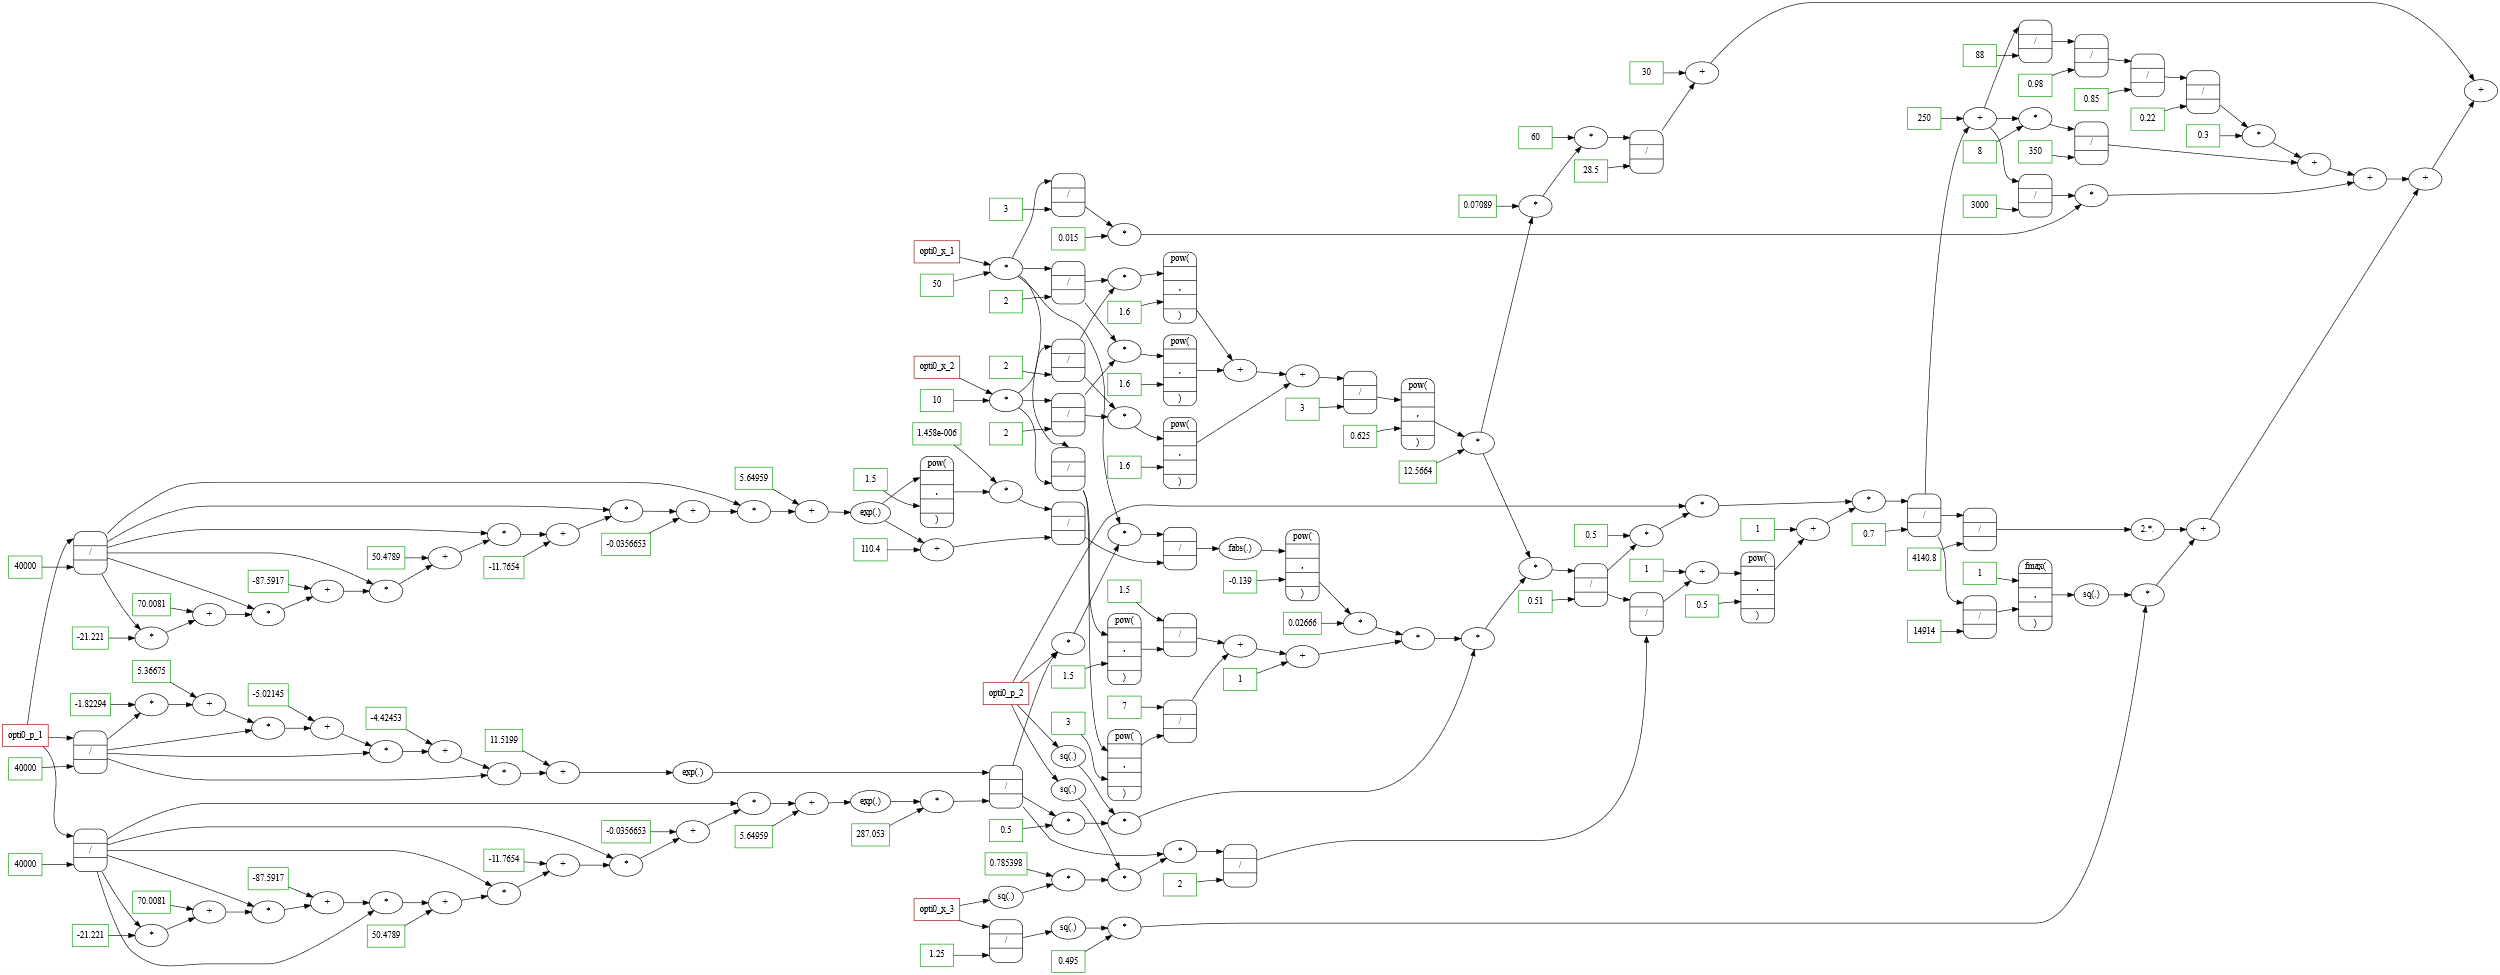
\includegraphics[width=\textwidth]{../figures/computational_graph_blimp.png} % TODO update
    \caption{Computational graph of a mass model for an airship, as constructed by AeroSandbox. This graph is automatically constructed at runtime.}
    \label{fig:computational-graph-aerosandbox}
\end{figure}

Once the graph is constructed, various user-specified inputs and outputs are connected to form a data structure representing a numerical optimization problem. With this information, code transformations can be applied. Most transformations, like automatic differentiation, automated sparsity detection, and problem scaling, are performed automatically and transparently to the user. Here, sensible default heuristics tuned on engineering design optimization problems are used. For example, the framework will automatically choose between forward-mode and reverse-mode automatic differentiation based on the size of the problem and the number of design variables. Likewise, problem scaling is applied on variables and constraints with a heuristic based on the user-provided initial guess, any bounds constraints, and the constraint Jacobian at the initial guess.

After appropriate code transformations are applied, the transformed problem is then solved using a numerical optimization backend. By default, this backend sends the solve to IPOPT \cite{wachter_implementation_2006}, a primal-dual interior point algorithm that performs favorably in large-scale engineering design optimization \cite{lyu_benchmarking_2014}. This core mathematical framework architecture, tradeoffs, and heuristics are discussed in further detail in prior work by Sharpe \cite{sharpe_aerosandbox_2021}.

This core design optimization framework is intended to be broadly applicable to many kinds of large-scale engineering systems. However, on top of this code framework, many optional aircraft-design-specific tools and physics modules are included, which make the framework especially well-suited to support these applications. These specialized tools are the focus of Chapter \ref{chap:physics}, though an overview of how these tools fit into the broader framework is given in Figure \ref{fig:asb-diagram}.

\begin{figure}[h]
    \centerline{\providecommand\ntxt{}
\renewcommand{\ntxt}[2]{
    \textbf{#1}\\#2
}

\tikzstyle{int} = [
thick,
rectangle, rounded corners, minimum height=2em,
draw=c1,  fill=c1!20,
text width=11em, text centered,
]
\tikzstyle{ext} = [int, draw=c2, fill=c2!20]
\tikzstyle{line} = [draw, thick, ->, shorten >=2pt, shorten <=2pt]

\begin{tikzpicture} [
    auto,
    node distance = 0.8cm and 0.8cm,
]
    \node (opti) [int] {\ntxt{ASB Core: \texttt{Opti} Stack}{Optimization interface}};
    \node (num) [int, right=of opti] {\ntxt{ASB Core: Numerics}{Unified numerics stack}};
    \node (cas) [ext, below=of opti] {\ntxt{CasADi or JAX \cite{casadi, jax}}{Computational graph framework}};
    \node (numpy) [ext, right=of cas] {\ntxt{NumPy \cite{numpy}}{Pre-computed numerics}};
    \node (ipopt) [ext, below=of cas] {\ntxt{IPOPT \cite{ipopt}}{Optimizer}};
    \node (surr) [int, above=of opti] {\ntxt{ASB Surrogate Modeling Tools}{}};
    \node (geom) [int, right=of surr] {\ntxt{ASB Geometry Stack}{}};
    \node (suge) at ($(surr)!0.5!(geom)$) {};
    \node (disc) [int, above=of suge, yshift=5pt] {\ntxt{ASB Discipline-Specific Tools}{}};

    \node (ldummy) [xshift=-0.5cm] at (opti.west) {};
    \node (rdummy) [xshift=0.5cm] at (num.east) {};

    % connect all nodes defined above
    \begin{scope} [every path/.style=line]
        \path (disc) -- (geom);
%        \path (disc) edge[out=180, in=180] (opti);
        \path [rounded corners] (disc) -| (ldummy.center) -- (opti);
%        \path (disc) edge[out=0, in=0] (num);
        \path [rounded corners] (disc) -| (rdummy.center) -- (num);
        \path (surr) -- (opti);
        \path (surr) -- (num);
        \path (geom) -- (num);
        \path (opti) -- (cas);
        \path (num) -- (cas);
        \path (num) -- (numpy);
        \path (cas) -- (ipopt);
        \path (opti) -- (num);
    \end{scope}

%    % Legend
%    \matrix [draw,below left] at (current bounding box.north east) {
%        \node [int, label=right:{AeroSandbox Component}]; \\
%        \node [ext, label=right:{External Library}]; \\
%    };

    \begin{scope} [xshift=9.5cm, yshift=-0.5cm, scale=4.5]
        \draw[black!75, <->] (0, -1.1) -- (0, 1.1);
        \foreach \y in {-1, -0.67, -0.33, 0, 0.33, 0.67, 1}
        \draw[shift={(0,\y)},color=black!75] (1pt,0pt) -- (-1pt, 0pt);
        \node[anchor=west,text width = 3cm](top) at (0.05, 1){More\\ abstract};
        \node[anchor=west,text width = 3cm](bot) at (0.05, -1){More\\ foundational};
    \end{scope}

\end{tikzpicture}}
    \caption{Dependency relationships between \textbf{\textcolor{c1!80!black}{AeroSandbox (ASB) components}} and \textbf{\textcolor{c2!80!black}{external libraries}}. Arrows point toward dependencies. Adapted from prior work by Sharpe \cite{sharpe_aerosandbox_2021}.}
    \label{fig:asb-diagram}
\end{figure}


\section{Performance Comparisons}

To test the hypothesis shown in Table \ref{tab:paradigm_comparison}, where a code transformations paradigm can offer a favorable compromise between ease-of-use and computational performance, we have conducted a series of benchmarking studies. Each benchmark is designed to compare performance on one of the three key practical metrics, and against at least one of the existing MDO paradigms listed in Table \ref{tab:paradigm_comparison}. % TODO cleanup

\subsection{Code Transformations vs. Black-Box Optimization Methods}

\subsection{Code Transformations vs. Disciplined Optimization Methods}

\subsection{Code Transformations vs. Analytic-Gradient Methods}


\section{Syntax Considerations}

\subsection{Procedural Coding Style}


\section{Aircraft Design Case Studies}

% Spiral development process

\subsection{Firefly} % TODO name

\subsection{Dawn} % TODO name

\subsection{Other Case Studies} % TODO name


\section{Computational Reproducibility}

%The code is made available open-source on GitHub under the permissive MIT license in order to gather as much practical user feedback as possible.


\section{Results-To-Date in Code Transformations}



AeroSandbox can be used to demonstrate the potential of code transformations to accelerate optimization problems with minimal effort. Here, we give an example comparison using the Rosenbrock optimization problem. This problem is a classic optimization benchmark, designed to be a stress-test as the optimum lies at the bottom of a shallow-curving valley \cite{rosenbrock}. Here, we solve an $N$-dimensional extension of this problem, which conveniently gives a knob to dial up or down the difficulty of the problem \cite{kok}. This optimization problem is defined in Equation \ref{eq:rosenbrock}:

\begin{mini}
    |l|
        {\vec{x}}{ \sum_{i=1}^{N-1} \left[ 100 \left(x_{i+1} - x_i^2 \right)^2 + \left(1 - x_i \right)^2 \right] }
        {}{}
%        \addConstraint{}
    \label{eq:rosenbrock}
\end{mini}

Figure \ref{fig:rosenbrock} illustrates this optimization landscape for the case where $N=2$, showing the curved valley. For all $N$, the global optimum is at $\vec{x} = \vec{1}$, where the objective function evaluates to $0$. This problem is chosen here because it shares many difficult aspects with engineering design optimization problems: it is nonlinear, nonconvex, and poorly-scaled. Furthermore, we deliberately choose poor initial guesses, with each element of the vector of initial guesses drawn from a random uniform distribution in the interval $[-10, 10]$.

\begin{figure}[H]
    \centering
    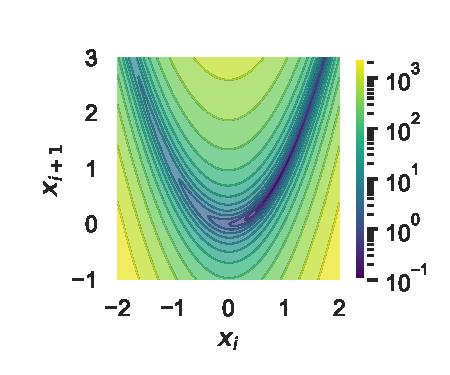
\includegraphics{../figures/rosenbrock_function.pdf}
    \caption{The Rosenbrock function, a classic optimization benchmark problem.}
    \label{fig:rosenbrock}
\end{figure}

In Figure \ref{fig:aerosandbox_scaling_comparison}, the performance of AeroSandbox (which leverages code transformations) is compared against existing methods using black-box optimization techniques. AeroSandbox offers faster practical and asymptotic optimization performance than existing black-box optimization methods, demonstrating the magnitude of acceleration that is possible with code transformations.

\begin{figure}[H]
    \centering
    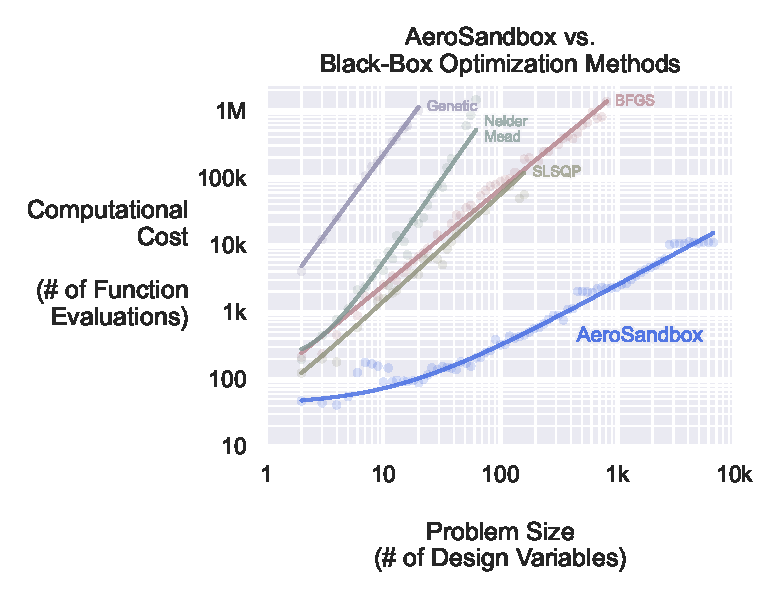
\includegraphics[width=0.8\textwidth]{../figures/benchmark_nd_rosenbrock.pdf}
    \caption{Comparison of optimization performance between AeroSandbox and existing black-box optimization methods on the $N$-dimensional Rosenbrock problem. Other methods are a Nelder-Mead simplex method and two gradient-based methods (SLSQP and BFGS), both using common SciPy implementations \cite{scipy}.}
    \label{fig:aerosandbox_scaling_comparison}
\end{figure}

Engineering benchmarks comparing the performance of an early implementation of the code transformations paradigm to disciplined optimization methods are given in Sharpe \cite{sharpe_aerosandbox_2021}. In short, code transformations can equal or exceed the performance of disciplined optimization methods such as geometric programming, even on problems where this disciplined optimization approach is applicable. This is a promising result, as it suggests that code transformations may be able to offer the best of both worlds on engineering problems: the computational performance of disciplined optimization methods without the strict mathematical restrictions.
